\documentclass[twoside]{supsistudent} 

% per settare noindent
\setlength{\parindent}{0pt}


% Crea un capitolo senza numerazione che pero` appare nell'indice %
\newcommand{\problemchapter}[1]{%
  \chapter*{#1}%
  \addcontentsline{toc}{chapter}{#1}%
\markboth{#1}{#1}
}

% Numerazione delle appendici secondo norma
\addto\appendix{
\renewcommand{\thesection}{\Alph{chapter}.\arabic{section}}
\renewcommand{\thesubsection}{\thesection.\arabic{subsection}}}

\setcounter{secnumdepth}{5} 	%per avere più livelli nei titoli
\setcounter{tocdepth}{5}		%per avere più livelli nell'indice


\titolo{App mobile per gestione timbrature e controllo qualità collaboratori}
\studente{Walter Sostene Losa}
\relatore{Andrea Baldassari}
\correlatore{Matteo Besenzoni}
\committente{Progect SA - Impresa Generale di Pulizie e Facility Management}
\corso{Ingegneria Informatica}
\codice{C10793}
\anno{2023/2024}



\begin{document}

\pagenumbering{alph}
\maketitle
\onehalfspacing
\frontmatter


\pagenumbering{roman}
\tableofcontents
\listoffigures					% Opzionale
\listoftables					% Opzionale

\newpage
\mainmatter
\pagenumbering{arabic}
\setcounter{page}{1}

\chapter*{Abstract}

\chapter{Progetto Assegnato}

Il partner di progetto, un'importante azienda attiva nei servizi di pulizia e facility management, necessita di un sistema che permetta la gestione e il controllo qualità dei servizi erogati presso i clienti. Il sistema, accessibile tramite applicazione mobile, sarà utilizzato principalmente da tre attori: Dipendenti, Responsabili e Clienti.

\section{Funzionalità per i Dipendenti}

I Dipendenti avranno a disposizione le seguenti funzionalità:
\begin{itemize}
  \item \textbf{Registrazione delle presenze}: I dipendenti possono registrare (timbrare) il loro arrivo e la loro partenza presso i clienti da cui si recano, tramite QR code o tag NFC dedicato.
  \item \textbf{Segnalazioni di anomalie}: Possono fare segnalazioni, allegando anche foto e video, presso i clienti, in caso di anomalie riscontrate durante il servizio.
  \item \textbf{Ordini di attrezzature e prodotti}: Possono fare un ordine delle attrezzature e dei prodotti che sono finiti o che sono in esaurimento, facilitando la gestione del materiale necessario per svolgere le loro mansioni.
\end{itemize}

\section{Funzionalità per i Responsabili}

I Responsabili avranno a disposizione le seguenti funzionalità:
\begin{itemize}
  \item \textbf{Verifica delle timbrature}: Possono verificare le timbrature dei dipendenti di loro responsabilità ai fini di controllo qualità, assicurando che i servizi vengano svolti nei tempi previsti.
  \item \textbf{Segnalazioni di controllo qualità}: Possono fare segnalazioni per controllo qualità, direttamente al dipendente ed indicando il cliente, permettendo una rapida risoluzione di eventuali problemi riscontrati.
\end{itemize}

\section{Funzionalità per i Clienti}

I Clienti avranno a disposizione le seguenti funzionalità:
\begin{itemize}
  \item \textbf{Segnalazioni di criticità}: Possono segnalare criticità nel servizio ricevuto, offrendo un feedback diretto all'azienda per migliorare la qualità del servizio.
  \item \textbf{Sondaggi sulla qualità del servizio}: Possono essere sottoposti a sondaggi sulla qualità del servizio ricevuto, fornendo dati utili per il miglioramento continuo.
\end{itemize}

\section{Obiettivi del Sistema}

Il sistema è progettato per raggiungere i seguenti obiettivi:
\begin{itemize}
  \item \textbf{Miglioramento della gestione delle presenze}: Tramite l'uso di tecnologie come QR code e tag NFC, il sistema assicura una registrazione precisa e affidabile delle presenze dei dipendenti.
  \item \textbf{Aumento della trasparenza e della comunicazione}: Le funzionalità di segnalazione per dipendenti, responsabili e clienti aumentano la trasparenza e migliorano la comunicazione tra le parti coinvolte.
  \item \textbf{Ottimizzazione delle risorse}: La possibilità di ordinare attrezzature e prodotti direttamente tramite l'app facilita la gestione delle risorse, assicurando che i dipendenti abbiano sempre a disposizione il materiale necessario.
  \item \textbf{Controllo qualità continuo}: Le funzionalità di verifica e segnalazione per i responsabili permettono un controllo qualità continuo, garantendo un elevato standard del servizio erogato.
\end{itemize}


\chapter{Introduzione}

Il progetto nasce dalla necessità di Progect SA, un'importante azienda attiva nei servizi di pulizia e facility management, di migliorare la gestione e il controllo qualità dei servizi erogati presso i clienti. L'azienda desidera un sistema che permetta ai dipendenti di registrare le presenze presso i clienti, di segnalare anomalie riscontrate durante il servizio e di fare ordini di attrezzature e prodotti. I responsabili devono poter verificare le timbrature dei dipendenti di loro responsabilità e fare segnalazioni per controllo qualità. I clienti devono poter segnalare criticità nel servizio ricevuto e essere sottoposti a sondaggi sulla qualità del servizio. Il sistema deve garantire una registrazione precisa e affidabile delle presenze, aumentare la trasparenza e migliorare la comunicazione tra le parti coinvolte, facilitare la gestione delle risorse e assicurare un controllo qualità continuo.\\
\\
Il sistema sarà accessibile tramite applicazione mobile e sarà utilizzato principalmente da tre attori: Dipendenti, Responsabili e Clienti. I Dipendenti potranno registrare le presenze, fare segnalazioni di anomalie e fare ordini di attrezzature e prodotti. I Responsabili potranno verificare le timbrature dei dipendenti e fare segnalazioni per controllo qualità. I Clienti potranno segnalare criticità e essere sottoposti a sondaggi sulla qualità del servizio.\\
\\
Il Capitolo 2 del documento presenta un’analisi delle motivazioni e del contesto che hanno guidato lo sviluppo del progetto. Inoltre, vengono introdotti in modo preliminare gli obiettivi che costituiscono il nucleo centrale di questo lavoro.\\
\\
todo: aggiungere una breve spiegazione di ogni capitolo

\chapter{Motivazione e Contesto}

In questo capitolo, vengono descritte le motivazioni accademiche che stanno alla base di
questo lavoro di tesi, insieme al contesto in cui si inseriscono. In conclusione, vengono
delineati gli obiettivi che guidano lo sviluppo di questo progetto.\\
\\
Nell'ambito del corso di Bachelor in Ingegneria Informatica presso la Scuola Universitaria
Professionale della Svizzera Italiana (SUPSI), ogni studente si trova di fronte al compito di
completare un lavoro di diploma. Questo implica la scelta autonoma di un progetto tra quelli
proposti da diversi relatori. Tali progetti abbracciano una vasta gamma di settori, spaziando
tra software desktop standalone, applicazioni web, networking, intelligenza artificiale e molto
altro. Ogni studente è tenuto a sviluppare il progetto nel corso della stagione estiva, per poi
consegnarlo entro l'inizio di settembre. Lo scopo di questo progetto è applicare le tecniche,
le strategie e i metodi di sviluppo appresi durante i tre anni di studi del percorso di Bachelor.\\
\\
La scelta di svolgere questo particolare progetto è stata determinata da diversi fattori. In
particolare, l'opportunità di sviluppare un'applicazione web è stata considerata un modo
per scoprire meglio questo campo non essendo stato molto visto durante gli anni, offrendo
uno spazio ideale per l'applicazione delle competenze acquisite. L'uso di un framework
aggiornato, ha fornito un'opportunità unica per scoprire una nuova tecnologia ancora non molto
diffusa nei sfotware odierni.\\
\\
Il progetto è seguito dai relatori Baldassari Andrea e Matteo Besenzoni, entrambi docenti e ricer-
catori presso la SUPSI. In particolare, il docente Andrea Baldassari ha fornito i requisiti e le specifiche man mano che il lavoro procedeva.

\section{Obiettivo}
L'obiettivo di questo progetto è sviluppare un'applicazione web per la gestione delle timbrature
e il controllo qualità dei collaboratori di Progect SA. L'applicazione deve permettere ai
collaboratori di timbrare in entrata e in uscita, di inserire le attività svolte durante la giornata
e di caricare le foto dei lavori eseguiti. Inoltre, l'applicazione deve permettere ai responsabili
di controllo qualità di visualizzare le timbrature e le attività svolte dai collaboratori, di
valutare la qualità del lavoro svolto e di fornire feedback ai collaboratori.\\
\\

\chapter{Problema}
Il problema affrontato nel contesto del progetto riguarda la necessità di sviluppare un sistema completo per la gestione delle timbrature e il controllo della qualità dei servizi offerti da un'azienda attiva nel settore della pulizia e del facility management. Attualmente, l'azienda si trova a dover affrontare diverse sfide legate alla gestione e al monitoraggio dei propri collaboratori e dei servizi erogati, tra cui:

\begin{itemize}
  \item \textbf{Mancanza di un sistema di tracciamento efficiente}: L'assenza di un sistema integrato per la registrazione delle timbrature dei dipendenti presso i vari clienti rende difficile il monitoraggio in tempo reale delle attività lavorative e il controllo della qualità dei servizi erogati.

  \item \textbf{Difficoltà nella gestione delle segnalazioni}: Attualmente, le segnalazioni relative a anomalie o criticità del servizio devono essere gestite manualmente, il che comporta inefficienze operative e ritardi nella risoluzione dei problemi.

  \item \textbf{Carenza di trasparenza nelle comunicazioni}: I canali di comunicazione tra dipendenti, responsabili e clienti non sono ottimizzati, portando a una scarsa trasparenza e a possibili incomprensioni riguardo alle prestazioni del servizio e alle necessità dei clienti.

  \item \textbf{Inadeguatezza nella gestione delle scorte di attrezzature e prodotti}: La mancanza di un sistema automatizzato per la gestione delle richieste di rifornimento di attrezzature e prodotti può causare ritardi nel rifornimento, con conseguente impatto negativo sulla qualità del servizio.

  \item \textbf{Limitazioni nell'integrazione tecnologica}: L'integrazione con dispositivi mobili e tecnologie come NFC e QR code non è stata pienamente sfruttata, limitando la possibilità di utilizzare strumenti digitali avanzati per il controllo della qualità e la gestione delle attività lavorative.

\end{itemize}


\chapter{Approccio al problema}
In questo capitolo, esamineremo in dettaglio l'approccio adottato per sviluppare una Progressive Web App (PWA) dedicata alla gestione e al controllo qualità dei servizi di pulizia e facility management. Illustreremo le scelte effettuate per quanto riguarda la gestione del progetto, i linguaggi di programmazione, i framework selezionati e l'integrazione con i componenti dei dispositivi mobili. Ogni decisione tecnica è stata presa con l'obiettivo di garantire prestazioni elevate, facilità di manutenzione e un'esperienza utente ottimale.

\section{Gestione del progetto}

La gestione del progetto è stata condotta utilizzando una metodologia Agile, in particolare il framework Scrum. Questa scelta è stata dettata dalla necessità di mantenere un'elevata flessibilità durante lo sviluppo, permettendo al team di adattarsi rapidamente ai cambiamenti nei requisiti del cliente. Ogni settimana è stato condotto uno sprint, al termine del quale si teneva una riunione con i committenti per presentare i progressi attraverso demo, raccogliere feedback e pianificare le attività per la settimana successiva.

Per la gestione del codice sorgente e delle attività del progetto, è stata utilizzata la piattaforma GitLab. GitLab ha offerto strumenti integrati per il versionamento del codice, la gestione delle issue, la pianificazione degli sprint e l'integrazione continua. Questi strumenti hanno facilitato una stretta collaborazione all'interno del team e una gestione efficace del progetto, assicurando che il codice fosse sempre aggiornato e che ogni membro del team fosse informato sugli sviluppi.

\section{Linguaggi di Programmazione}

\subsection{Backend}

Per lo sviluppo del backend, abbiamo scelto di utilizzare Node.js in combinazione con il framework Express e l'ORM Sequelize. La scelta di Node.js è stata guidata da diversi fattori chiave:

\begin{itemize}
  \item \textbf{Asincronicità e Performance}: Node.js è basato su un modello di I/O non bloccante, che consente di gestire un elevato numero di richieste simultanee con un'efficienza notevole. Questo è particolarmente vantaggioso per un'applicazione che deve interagire con dispositivi mobili e gestire numerose operazioni in tempo reale, come l'acquisizione di dati dai sensori dei dispositivi.
  \item \textbf{Ampio Ecosistema}: Node.js dispone di un vasto ecosistema di librerie e moduli disponibili attraverso npm (Node Package Manager). Questo ci ha permesso di accelerare lo sviluppo utilizzando pacchetti preesistenti per funzionalità comuni, riducendo il tempo necessario per implementare funzioni complesse.
  \item \textbf{Scalabilità}: La natura asincrona di Node.js lo rende particolarmente adatto per costruire applicazioni scalabili. Per un sistema come quello proposto, che potrebbe essere utilizzato da numerosi utenti contemporaneamente, la capacità di scalare orizzontalmente è cruciale.
\end{itemize}

Express, un framework minimalista per Node.js, è stato scelto per la sua semplicità e flessibilità nella gestione delle API RESTful. Express consente di strutturare l'applicazione in modo modulare, facilitando la manutenzione e l'espansione del codice nel tempo. Inoltre, con l'uso di Sequelize, un ORM per Node.js, è stato possibile gestire le interazioni con il database MySQL in modo sicuro ed efficiente, mappando le tabelle del database su oggetti JavaScript e semplificando le operazioni CRUD (Create, Read, Update, Delete).

\subsection{Frontend}

Per il frontend, è stato scelto React come framework principale per lo sviluppo dell'interfaccia utente. Le motivazioni alla base di questa scelta sono molteplici:

\begin{itemize}
  \item \textbf{Componentizzazione}: React adotta un approccio basato su componenti, che permette di costruire interfacce utente modulari e riutilizzabili. Questa modularità non solo facilita lo sviluppo, ma rende anche più semplice la manutenzione e l'aggiornamento dell'applicazione nel tempo.
  \item \textbf{Performance e Virtual DOM}: React utilizza un Virtual DOM per ottimizzare il rendering dell'interfaccia utente. Questo riduce al minimo le operazioni di manipolazione del DOM reale, migliorando le prestazioni, soprattutto su dispositivi mobili, dove la potenza di calcolo può essere limitata.
  \item \textbf{Ecosistema e Community}: La vasta community di React e l'ampio ecosistema di librerie di supporto hanno fornito strumenti utili e best practices che hanno accelerato lo sviluppo e migliorato la qualità del codice.
\end{itemize}

Inoltre, per migliorare ulteriormente la velocità di sviluppo e la coerenza dell'interfaccia utente, è stata utilizzata la libreria \textbf{Ant Design (Antd)}. Antd è un set di componenti UI predefiniti per React, che offre una vasta gamma di elementi grafici stilisticamente coerenti e pronti all'uso. L'adozione di Antd ha permesso al team di:

\begin{itemize}
  \item \textbf{Accelerare lo Sviluppo}: Utilizzando componenti predefiniti di alta qualità, il team ha potuto concentrarsi maggiormente sulle logiche di business piuttosto che sulla progettazione e implementazione di elementi grafici complessi.
  \item \textbf{Mantenere una UI Coerente}: Antd garantisce che l'interfaccia utente sia esteticamente coerente e intuitiva, migliorando l'esperienza utente complessiva.
  \item \textbf{Facile Personalizzazione}: Sebbene Antd offra componenti predefiniti, è altamente personalizzabile, consentendo al team di adattare l'aspetto e il comportamento dei componenti alle specifiche esigenze del progetto.
\end{itemize}

L'uso di React, insieme a Antd, ha inoltre facilitato l'integrazione con le API dei dispositivi, come la fotocamera e i sensori di posizione, rendendo possibile la realizzazione di funzionalità critiche come la scansione di QR code e la tracciabilità GPS.

\section{Integrazione con Componenti del Dispositivo}

Uno degli aspetti più innovativi dell'applicazione è la sua capacità di interagire direttamente con i componenti hardware dei dispositivi mobili. Grazie a librerie specifiche di React, l'applicazione può accedere alla fotocamera per scattare foto e scansionare codici QR, nonché raccogliere dati GPS per tracciare la posizione dei lavoratori in tempo reale. Questo livello di integrazione è stato fondamentale per garantire che il sistema potesse offrire funzionalità di controllo qualità avanzate, come la verifica dell'ubicazione del personale sul campo e la documentazione delle attività svolte.

\section{Toolkits}

Oltre ai linguaggi e framework descritti, sono stati utilizzati diversi toolkits per supportare lo sviluppo:

\begin{itemize}
  \item \textbf{npm}: Il gestore di pacchetti npm è stato fondamentale per la gestione delle dipendenze e per l'installazione di librerie esterne che hanno velocizzato lo sviluppo.
  \item \textbf{Webpack}: Webpack è stato utilizzato per il bundling dei file JavaScript, ottimizzando le performance del frontend e migliorando i tempi di caricamento dell'applicazione.
  \item \textbf{GitLab CI/CD}: La pipeline CI/CD di GitLab ha automatizzato il processo di testing e deployment, garantendo che ogni modifica al codice fosse adeguatamente verificata prima di essere distribuita nell'ambiente di produzione.
\end{itemize}

L'insieme di questi strumenti ha permesso di creare un ambiente di sviluppo efficiente e affidabile, facilitando il rilascio continuo di nuove funzionalità e miglioramenti.

\chapter{Progettazione}

In questo capitolo viene descritta la fase di progettazione dell’applicativo, partendo dall'analisi dei requisiti necessari per poi passare alla descrizione delle funzionalità principali e dei mockup delle interfacce che saranno utilizzate dagli utenti.

\section{Requisiti}

Il sistema, accessibile tramite app, avrà principalmente quattro tipi di utenti: amministratori, dipendenti, responsabili (supervisori), e clienti. Di seguito sono elencati i requisiti specifici per ciascuno di questi ruoli.

\subsection{Requisiti per gli Amministratori}

Gli amministratori hanno il compito di gestire l'intero sistema, comprese le operazioni di gestione utenti e forniture. I requisiti specifici per questo ruolo includono:

\begin{itemize}
  \item Creare, modificare e gestire gli account degli utenti (dipendenti, responsabili e clienti).
  \item Aggiungere, modificare e gestire le forniture disponibili nel database.
  \item Monitorare tutte le segnalazioni di controllo qualità effettuate dai clienti.
  \item Visualizzare e gestire tutti i servizi svolti dai dipendenti.
\end{itemize}

\subsection{Requisiti per i Dipendenti}

I dipendenti sono coloro che eseguono le attività operative presso i clienti. I requisiti specifici per questo ruolo includono:

\begin{itemize}
  \item Registrare (timbrare) il loro arrivo e la loro partenza presso i clienti utilizzando QR code.
  \item Effettuare segnalazioni in caso di anomalie riscontrate presso i clienti.
  \item Ordinare attrezzature e prodotti che sono finiti o in esaurimento.
\end{itemize}

\subsection{Requisiti per i Responsabili (Supervisori)}

I responsabili, che sono dipendenti con funzioni aggiuntive, hanno il compito di controllare la qualità del lavoro svolto dai dipendenti sotto la loro responsabilità. I requisiti specifici per questo ruolo includono:

\begin{itemize}
  \item Verificare le timbrature dei dipendenti di loro responsabilità ai fini del controllo qualità.
\end{itemize}

\subsection{Requisiti per i Clienti}

I clienti sono coloro che ricevono i servizi e possono fornire feedback sulla loro qualità. I requisiti specifici per questo ruolo includono:

\begin{itemize}
  \item Segnalare criticità nel servizio ricevuto.
\end{itemize}


\section{Mockup delle Interfacce}

In questa sezione vengono descritti i mockup delle interfacce dell’applicazione, con particolare attenzione alle schermate più rilevanti per ciascun attore coinvolto (dipendenti, responsabili e clienti).

\subsection{Pagina di accesso}
\subsection{Pagina di registrazione delle timbrature}
\subsection{Pagina di gestione delle segnalazioni}
\subsection{Pagina di controllo qualità per i responsabili}
\subsection{Pagina di feedback dei clienti}



\chapter{Architettura}

In questo capitolo viene descritta l’architettura dell’applicativo. Iniziando con una visione generale di come sia strutturato l’applicativo, per poi passare ad una descrizione della struttura del codice, successivamente una spiegazione su come frontend e backend interagiscono tra di loro e come il backend comunica con il database.

\section{Visione Generale}

L'applicazione è progettata con un'architettura a componenti separati, suddivisa in tre parti principali:

\begin{itemize}
  \item \textbf{Frontend}: Fornisce un'interfaccia intuitiva e interattiva per l'interazione con il sistema.
  \item \textbf{Backend}: Gestisce le richieste dal frontend, elabora i dati e comunica con il database.
  \item \textbf{Database MySQL}:Utilizzato per la persistenza dei dati, come informazioni sugli utenti, accessi e servizi.
\end{itemize}

%aggiungere schema visione generale


\section{Struttura del Codice}
In questa sezione vengono discusse le scelte e le motivazioni che hanno portato a definire la struttura del codice dell’applicativo

\subsection{Frontend}
Lo sviluppo del frontend si è basato su convenzioni comuni utilizzate per sviluppare in \textit{TypeScript} e \textit{React}.
\\\\
All'interno della cartella \texttt{frontend} è dunque presente una cartella \texttt{src} la quale contiene tutto il codice dell'applicativo web.

La cartella viene poi suddivisa in:

\begin{itemize}
  \item \texttt{components}: collezione di componenti utilizzati all'interno dell'applicazione.
  \item \texttt{services}: collezione di servizi utilizzati per comunicare con il backend.
  \item \texttt{context}: collezione di contesti utilizzati per gestire lo stato dell'applicazione.
  \item \texttt{pages}: diverse pagine alle quali si può accedere attraverso l'applicazione.
  \item \texttt{utils}: file di utilità contenenti funzioni utilizzate più volte all'interno del frontend.
\end{itemize}

Oltre alle cartelle sopra elencate, sono presenti anche i file \texttt{App.tsx} e \texttt{index.tsx} i quali rappresentano rispettivamente il componente principale dell'applicazione e il file di entry point.
\\\\
Infine è presente anche un file chiamato \texttt{type.ts} il quale contiene tutte le interfacce utilizzate all'interno del frontend.

\subsection{Backend}
Il progetto di backend è stato scritto in \textit{Node.js} utilizzando il framework \textit{Express}. Questo ha permesso di creare un server web che gestisce le richieste HTTP provenienti dal frontend e comunica con il database per recuperare e salvare i dati.\\

All'interno della cartella \texttt{backend} è presente una cartella \texttt{src} la quale contiene tutto il codice del server. In particolare, la cartella è suddivisa in:
\begin{itemize}
  \item \texttt{db}: contiene i modelli e le configurazioni del database.
  \item \texttt{middleware}: contiene i middleware utilizzati per gestire le richieste HTTP.
  \item \texttt{repositories}: contiene i repository utilizzati per interagire con il database.
  \item \texttt{resources}: contiene le risorse che vengono inviate al frontend.
  \item \texttt{routes}: contiene i controller che gestiscono le richieste HTTP.
  \item \texttt{utils}: file di utilità contenenti funzioni utilizzate più volte all'interno del backend.
\end{itemize}

Anche in questo caso, oltre alle cartelle sopra elencate, sono presenti i file \texttt{app.ts} e \texttt{server.ts} i quali rappresentano rispettivamente il componente principale del server e il file di entry point.

\section{Comunicazione Frontend-Backend}
In questa sezione viene descritta l'interazione tra il frontend e il backend dell'applicazione, illustrando il flusso di comunicazione e le tecnologie utilizzate per garantire un'efficace integrazione tra i due componenti.

\subsection{Comunicazione tramite API REST}

Il frontend e il backend comunicano principalmente tramite API REST (Representational State Transfer). Le API REST sono endpoint esposti dal backend che il frontend può chiamare per inviare o ricevere dati. Questi endpoint sono progettati per seguire i principi REST, che includono l'uso di metodi HTTP standard come GET, POST, PUT e DELETE per operazioni CRUD (Create, Read, Update, Delete).

\begin{itemize}
  \item \textbf{GET}: Utilizzato per recuperare dati dal backend. Ad esempio, il frontend può effettuare una richiesta GET per ottenere una lista di servizi o dettagli su un utente specifico.
  \item \textbf{POST}: Utilizzato per inviare nuovi dati al backend. Ad esempio, quando un utente registra una nuova timbratura, il frontend invia una richiesta POST al backend con i dettagli della timbratura.
  \item \textbf{PUT}: Utilizzato per aggiornare dati esistenti nel backend. Ad esempio, il frontend può inviare una richiesta PUT per aggiornare le informazioni di un servizio esistente.
  \item \textbf{DELETE}: Utilizzato per eliminare dati dal backend. Ad esempio, il frontend può effettuare una richiesta DELETE per rimuovere un utente.
\end{itemize}

\subsection{Struttura delle Richieste e Risposte}

Le richieste dal frontend al backend sono effettuate utilizzando la libreria \texttt{axios}. Ogni richiesta include un URL di destinazione (l'endpoint dell'API), un metodo HTTP, e, se necessario, un corpo della richiesta (payload) con i dati da inviare.

Le risposte del backend possono includere dati in formato JSON (JavaScript Object Notation) o oggetti JavaScript. Le risposte includono un codice di stato HTTP che indica l'esito dell'operazione (ad esempio, 200 OK, 404 Not Found, 500 Internal Server Error) e, se applicabile, i dati richiesti o un messaggio di errore.

\begin{itemize}
  \item \textbf{Richiesta GET}: Il frontend invia una richiesta GET all'endpoint \texttt{/api/users} per recuperare la lista degli utenti. Il backend risponde con una Collection di UserResource contenente i dati degli utenti.
  \item \textbf{Richiesta POST}: Il frontend invia una richiesta POST all'endpoint \texttt{/api/time-tracking/new-time} con i dettagli della timbratura. Il backend elabora i dati e restituisce un JSON con un messaggio di conferma.
  \item \textbf{Richiesta PUT}: Il frontend invia una richiesta PUT all'endpoint \texttt{/api/time-tracking/stop-time/\$timeTrackingId} per aggiornare i dettagli di un servizio con ID timeTrackingId. Il backend aggiorna il servizio con i dati aggiornati.
  \item \textbf{Richiesta DELETE}: Il frontend invia una richiesta DELETE all'endpoint \texttt{/api/users/\$id} per eliminare un utente con ID id. Il backend elimina l'utente e restituisce una conferma di eliminazione.
\end{itemize}

\subsection{Gestione degli Errori e Feedback}

Durante la comunicazione tra frontend e backend, è essenziale gestire correttamente gli errori e fornire feedback agli utenti. Il backend deve restituire messaggi di errore chiari e informativi quando si verificano problemi, come dati non validi o errori di connessione.

Il frontend è responsabile della visualizzazione di questi messaggi di errore all'utente in modo chiaro e comprensibile.

\subsection{Autenticazione e Autorizzazione}

La comunicazione tra frontend e backend è protetta tramite meccanismi di autenticazione e autorizzazione. Il backend richiede che il frontend invii un token di autenticazione con ogni richiesta per verificare l'identità dell'utente e determinare i permessi di accesso.

Il frontend gestisce il processo di autenticazione, memorizza il token di autenticazione nei cookie, e lo include nelle intestazioni delle richieste successive. Questo garantisce che solo gli utenti autorizzati possano accedere a determinati endpoint e operazioni.

\subsection{Esempio di Flusso di Comunicazione}

\begin{enumerate}
  \item \textbf{Richiesta di Autenticazione}: L'utente inserisce le proprie credenziali nel frontend. Il frontend invia una richiesta POST all'endpoint \texttt{/api/login} con le credenziali.
  \item \textbf{Risposta di Autenticazione}: Il backend verifica le credenziali e, se valide, restituisce un token di autenticazione.
  \item \textbf{Richiesta Dati Utente}: Nelle prossime richieste, il frontend include il token di autenticazione nelle intestazioni. Ad esempio, il frontend invia una richiesta GET all'endpoint \texttt{/api/user} per ottenere i dettagli del profilo utente.
  \item \textbf{Risposta Dati Utente}: Il backend verifica il token prima di restituire i dati del profilo utente. Se il token è valido, il backend restituisce i dati richiesti.
\end{enumerate}

Questo flusso di comunicazione assicura che il frontend e il backend lavorino insieme in modo sinergico, offrendo un'esperienza utente fluida e sicura.

\subsection{Sicurezza nella Gestione dei Dati Sensibili}

La sicurezza dei dati sensibili, come le password degli utenti, è una priorità assoluta nel sistema. Durante la comunicazione tra frontend e backend, i dati sensibili vengono protetti attraverso diversi meccanismi di sicurezza.

Le password degli utenti non vengono mai trasmesse in chiaro. Quando un utente invia la propria password tramite il frontend, questa viene inviata al backend utilizzando una connessione sicura tramite HTTPS (Hypertext Transfer Protocol Secure). HTTPS crittografa i dati in transito, rendendo estremamente difficile per eventuali malintenzionati intercettare o manipolare le informazioni trasmesse.

Nel backend, le password non vengono mai memorizzate in formato leggibile. Al momento della registrazione o dell'aggiornamento della password, il backend utilizza la libreria \texttt{bcrypt} per eseguire l'hashing della password. L'hashing è un processo che trasforma la password in una stringa di caratteri crittografata. Ad esempio, la seguente istruzione \texttt{bcrypt.hash(body.pw, 12)} genera un hash della password con un cost factor di 12, aumentando così la complessità computazionale richiesta per un eventuale attacco di forza bruta.

\begin{itemize}
  \item \textbf{Hashing}: Quando il backend riceve la password in chiaro dal frontend, questa viene immediatamente sottoposta a un processo di hashing utilizzando l'algoritmo bcrypt. Questo processo assicura che la password originale non sia mai memorizzata nel database. Al suo posto, viene salvato solo l'hash della password.

  \item \textbf{Verifica della Password}: Quando un utente tenta di effettuare il login, il backend confronta la password inviata dal frontend con l'hash memorizzato nel database utilizzando il metodo \texttt{bcrypt.compare}. Se la password corrisponde all'hash memorizzato, l'autenticazione viene considerata valida.
\end{itemize}

Grazie a questo approccio, anche in caso di compromissione del database, le password degli utenti rimangono protette, poiché gli hash sono difficili da invertire. Inoltre, il cost factor di bcrypt, configurabile nel codice (in questo caso impostato a 12), assicura che il processo di hashing sia sufficientemente lento da rendere inefficaci gli attacchi basati su tecniche di brute force.


\section{Comunicazione Backend-Database}

La comunicazione tra il backend e il database avviene principalmente attraverso query SQL, che vengono generate ed eseguite dal backend per interagire con il database MySQL. Questa interazione consente al backend di gestire dati persistenti, come informazioni sugli utenti, le timbrature e i dettagli dei servizi.

Per facilitare e semplificare le operazioni di accesso al database, è stato utilizzato un ORM (Object-Relational Mapping) chiamato \textbf{Sequelize}. Questo strumento permette di gestire il database tramite codice JavaScript, senza dover scrivere manualmente query SQL, semplificando quindi l'accesso ai dati e la loro manipolazione.

\subsection{Operazioni CRUD tramite ORM}

L'interazione backend-database segue principalmente i principi CRUD (Create, Read, Update, Delete), che rappresentano le operazioni di base per la gestione dei dati nel database.

\begin{itemize}
  \item \textbf{Create (Creare)}: Quando il backend riceve una richiesta per creare una nuova risorsa (come un nuovo utente o una nuova timbratura), esso utilizza Sequelize per generare la corrispondente query SQL di inserimento. Questa query viene poi eseguita nel database MySQL per aggiungere il nuovo record.

  \item \textbf{Read (Leggere)}: Il backend può inviare query di lettura al database per recuperare informazioni, come una lista di utenti o le timbrature di un dipendente. Sequelize converte le richieste di lettura del backend in query SQL SELECT, e i dati recuperati vengono restituiti come oggetti JavaScript pronti per essere utilizzati nel codice.

  \item \textbf{Update (Aggiornare)}: Per aggiornare informazioni già esistenti, come modificare il profilo di un utente o aggiornare lo stato di un servizio, il backend invia query SQL di aggiornamento al database. Sequelize gestisce queste operazioni di aggiornamento in modo sicuro, traducendo le modifiche in query SQL UPDATE, e garantendo che solo i campi necessari siano modificati.

  \item \textbf{Delete (Eliminare)}: Quando il backend deve rimuovere dati, ad esempio cancellare un utente o eliminare una segnalazione, Sequelize genera ed esegue query SQL DELETE che rimuovono i record dal database in modo sicuro.
\end{itemize}

\subsection{Gestione delle Relazioni tra Tabelle}

Uno dei vantaggi principali dell'utilizzo di un ORM come Sequelize è la capacità di gestire facilmente le relazioni tra le tabelle del database. Il sistema richiede la gestione di relazioni complesse tra diversi tipi di dati, come utenti, servizi e timbrature. Grazie a Sequelize, il backend può definire queste relazioni a livello di codice, rappresentando legami come "uno a molti" o "molti a molti".

Ad esempio:

\begin{itemize}
  \item \textbf{Relazione Uno-a-Molti}: Un amministratore può gestire molti dipendenti, e un dipendente può avere molte timbrature. Sequelize permette di rappresentare queste relazioni utilizzando associazioni tra modelli, come la relazione tra il modello "User" e il modello "TimeTracking".

  \item \textbf{Relazione Molti-a-Molti}: I clienti possono avere rapporti con più servizi, e ogni servizio può essere assegnato a più clienti. Questo tipo di relazione può essere gestito tramite tabelle ponte, che Sequelize crea e gestisce automaticamente.
\end{itemize}

\subsection{Validazione dei Dati e Gestione degli Errori}

Durante l'interazione con il database, è importante garantire che i dati siano validi e consistenti. Sequelize offre funzionalità di validazione automatica per assicurarsi che i dati inviati al database rispettino determinati vincoli, come tipi di dato corretti e la presenza di campi obbligatori.

Inoltre, Sequelize gestisce anche gli errori generati durante le operazioni con il database, come violazioni di vincoli di unicità o errori di connessione. Il backend cattura questi errori e li gestisce in modo appropriato, inviando feedback dettagliati al frontend.

\subsection{Sicurezza e Ottimizzazione delle Query}

Per garantire la sicurezza delle operazioni sul database, Sequelize include meccanismi per prevenire attacchi comuni, come l'SQL injection. Le query generate automaticamente da Sequelize sono parametrizzate, il che impedisce l'inserimento di comandi SQL malevoli all'interno delle query.

Inoltre, Sequelize è ottimizzato per generare query SQL efficienti, minimizzando l'impatto sulle prestazioni del sistema anche quando si gestiscono grandi quantità di dati. Per query più complesse o personalizzate, è comunque possibile eseguire query SQL raw (non processate) per ottenere maggiore controllo e precisione.

\subsection{Esempio di Flusso di Comunicazione}

\begin{enumerate}
  \item \textbf{Richiesta di Creazione Dati}: Quando un utente registra una nuova timbratura, il backend crea un nuovo record nel database utilizzando una query di inserimento generata da Sequelize.

  \item \textbf{Richiesta di Lettura Dati}: Il backend effettua una query di selezione per ottenere tutte le timbrature associate a un dipendente. Sequelize converte la richiesta del backend in una query SQL SELECT ed esegue la query sul database MySQL.

  \item \textbf{Risposta dal Database}: I dati vengono restituiti dal database sotto forma di oggetti JavaScript, che il backend invia al frontend.
\end{enumerate}

Questo flusso garantisce che il backend possa interagire in modo efficiente con il database per memorizzare e recuperare informazioni, mantenendo il sistema sicuro e performante.

\chapter{Implementazione}

Questo capitolo descrive in dettaglio il processo di implementazione dei vari componenti del progetto, fornendo una panoramica completa delle scelte progettuali e delle tecnologie utilizzate. Vengono analizzate sia la parte backend che quella frontend dell'applicazione, spiegando come ciascun componente è stato sviluppato per rispondere alle specifiche esigenze funzionali del sistema.
\section{Backend}
\subsection{Database}
Il database è organizzato secondo il paradigma relazionale e utilizza il sistema di gestione MySQL. Le entità principali sono rappresentate da tabelle che modellano utenti, tracciamenti temporali, forniture e feedback. La struttura delle tabelle e le relazioni tra di esse vengono gestite tramite Sequelize, un ORM (Object-Relational Mapping) che mappa le entità del database con modelli in JavaScript (Figura \ref{fig:databaseschema}).

\subsubsection{Tabelle e Modelli}
\begin{itemize}
  \item \textbf{User (Utenti)}: La tabella \texttt{users} rappresenta gli utenti del sistema, con campi come \texttt{id}, \texttt{name}, \texttt{email}, \texttt{pw} (password) e \texttt{role} (ruolo). I ruoli possono essere \texttt{admin}, \texttt{supervisor}, \texttt{employee} o \texttt{client}.
  \item \textbf{TimeTracking (Tracciamenti Temporali)}: La tabella \texttt{timetracking} rappresenta i tracciamenti temporali delle attività. Ogni record contiene i campi \texttt{id}, \texttt{employeeId}, \texttt{clientId}, \texttt{startTime}, \texttt{endTime}, \texttt{status} (stato dell'attività), e le coordinate di latitudine e longitudine di inizio e fine dell'attività.
  \item \textbf{Supply (Forniture)}: La tabella \texttt{supply} contiene le informazioni sulle forniture utilizzate durante un'attività. I campi principali includono \texttt{id}, \texttt{name}, e le date di creazione e aggiornamento.
  \item \textbf{Feedback}: La tabella \texttt{feedback} rappresenta i feedback forniti dai clienti. Include i campi \texttt{id}, \texttt{clientId}, e \texttt{notes}.
  \item \textbf{TimeTrackingSupply (Relazione tra Tracciamenti e Forniture)}: La tabella \texttt{timetracking\_supply} stabilisce una relazione molti-a-molti tra \texttt{TimeTracking} e \texttt{Supply}, collegando le forniture alle singole attività di tracciamento.
\end{itemize}

\subsubsection{Relazioni tra le Entità}
Le relazioni tra le tabelle sono implementate utilizzando le associazioni di Sequelize:
\begin{itemize}
  \item \texttt{User} ha una relazione uno-a-molti con \texttt{TimeTracking} sia come dipendente (\texttt{employee}) che come cliente (\texttt{client}).
  \item \texttt{TimeTracking} ha una relazione molti-a-molti con \texttt{Supply} attraverso la tabella di collegamento \texttt{TimeTrackingSupply}.
  \item \texttt{Feedback} ha una relazione uno-a-molti con \texttt{User} (come \texttt{client}).
\end{itemize}

\begin{figure}[ht]
  \centering
  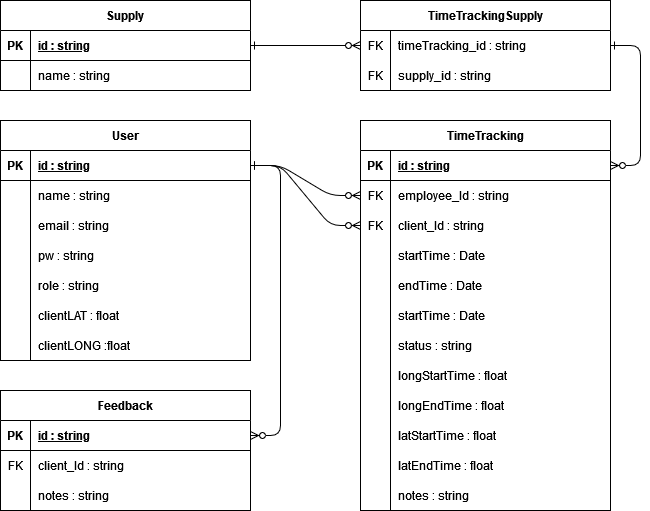
\includegraphics[scale=0.6]{./images/dbschema.png}
  \caption{Schema del Database.}
  \label{fig:databaseschema}
\end{figure}

\subsubsection{Gestione delle Date}
Ogni entità include i campi \texttt{created\_at} e \texttt{updated\_at}, che vengono gestiti automaticamente da Sequelize tramite l'opzione \texttt{timestamps: true}. Questo garantisce che ogni record mantenga una traccia delle date di creazione e aggiornamento.

\subsubsection{Implementazione della Sicurezza}
La sicurezza dei dati è garantita attraverso la configurazione delle credenziali e la gestione delle connessioni tramite variabili d'ambiente, mantenute in sicurezza utilizzando un manager delle variabili di ambiente (come mostrato nell'implementazione di \texttt{EnvManager}). L'applicazione utilizza inoltre CORS e un middleware di autenticazione tramite Passport per proteggere le API esposte.

\subsection{Collegamento tra Backend e Database}
Il collegamento tra il backend e il database è realizzato utilizzando \texttt{Sequelize}, un ORM (Object-Relational Mapping) che consente di mappare le entità del database su modelli JavaScript. Il backend è sviluppato in \texttt{Node.js} con l'ausilio della libreria \texttt{Express.js}, la quale fornisce un'infrastruttura per creare e gestire server HTTP.

\subsubsection{Architettura del Repository}
Il backend implementa un'architettura basata su repository, come mostrato dalla classe astratta \texttt{BaseRepository}. Questa classe definisce metodi generici per eseguire operazioni CRUD (Create, Read, Update, Delete) sul database, quali:
\begin{itemize}
  \item \texttt{getAll()}: Recupera tutte le istanze di un modello specifico dal database, consentendo anche di specificare opzioni di ordinamento.
  \item \texttt{getById()}: Recupera un'istanza specifica identificata dal suo \texttt{id}.
  \item \texttt{create()}: Crea una nuova istanza di un'entità e la salva nel database.
  \item \texttt{getByField()}: Cerca entità basate su un campo specifico e il suo valore.
  \item \texttt{update()}: Aggiorna un'istanza esistente.
  \item \texttt{delete()}: Elimina un'istanza specifica dal database.
\end{itemize}
Il collegamento tra il backend e il database avviene tramite il modello configurato in Sequelize, il quale è passato come parametro alla classe repository. \texttt{Sequelize} traduce le operazioni effettuate sui modelli in query SQL eseguite sul database.


\subsubsection{Inizializzazione del Server}
Il server viene creato utilizzando la funzione \texttt{createServer()}. Vengono applicati diversi middleware, tra cui:
\begin{itemize}
  \item \texttt{morgan}: Per il logging delle richieste HTTP.
  \item \texttt{cors}: Per la gestione delle richieste provenienti da domini esterni.
  \item \texttt{cookieParser}: Per il parsing dei cookie.
  \item \texttt{express.json()} e \texttt{express.urlencoded()}: Per il parsing dei dati del corpo delle richieste.
  \item \texttt{initializePassport()}: Per la gestione dell'autenticazione tramite Passport.js.
\end{itemize}
Dopo l'inizializzazione del server, viene esposta una rotta di health check (\texttt{/healthz}), la quale restituisce un semplice messaggio per confermare lo stato di salute del server e l'ambiente in cui sta girando (produzione o sviluppo).

\subsection{Percorsi API}

Il backend espone una serie di percorsi API (Tabella \ref{tab:api_routes}) attraverso il router definito nel file \texttt{routes}. Questo router gestisce le diverse rotte HTTP come \texttt{GET}, \texttt{POST}, \texttt{PUT} e \texttt{DELETE}, ciascuna delle quali è associata a una specifica funzione di controller. I controller sono responsabili dell'esecuzione delle operazioni richieste, come la lettura o la modifica dei dati nel database, attraverso l'utilizzo dei metodi definiti nei repository.

Le API sono progettate seguendo i principi REST, garantendo una struttura chiara e intuitiva. Ogni percorso è pensato per consentire al frontend di interagire in modo efficiente con il sistema, fornendo funzionalità come la gestione degli utenti, la registrazione delle timbrature e la creazione di segnalazioni. Questa architettura favorisce una comunicazione fluida tra frontend e backend, assicurando che le operazioni siano semplici da eseguire e coerenti con le best practice di sviluppo.


\begin{table}[h!]
  \resizebox{\textwidth}{!}{
    \begin{tabular}{|l|l|l|}
      \hline
      \textbf{HTTP Method} & \textbf{Route}                                              & \textbf{Descrizione}                                     \\ \hline
      POST                 & /auth/login                                                 & Gestice il login dell'utente.                            \\ \hline
      POST                 & /auth/logout                                                & Gestisce il logout dell'utente.                          \\ \hline
      GET                  & /users/                                                     & Ritorna la lista di utenti.                              \\ \hline
      POST                 & /users/                                                     & Crea un nuovo utente.                                    \\ \hline
      GET                  & /users/role/:role                                           & Ritorna la lista di utenti in base al ruolo.             \\ \hline
      GET                  & /users/:id                                                  & Ritorna un utente in base al suo ID univoco.             \\ \hline
      PUT                  & /users/:id                                                  & Modifica un utente in base al suo ID univoco.            \\ \hline
      DELETE               & /users/:id                                                  & Elimina un utente in base al suo ID univoco.             \\ \hline
      GET                  & /time-tracking/get-all-time                                 & Ritorna la lista di timbrature.                          \\ \hline
      POST                 & /time-tracking/new-time                                     & Crea una nuova timbratura.                               \\ \hline
      PUT                  & /time-tracking/stop-time/::id                               & Ferma una timbratura in base al suo ID univoco.          \\ \hline
      GET                  & /time-tracking/get-time/:id                                 & Ritorna una timbratura in base al suo ID univoco.        \\ \hline
      GET                  & /time-tracking/get-client-time/:clientId                    & Ritorna la lista di timbrature di un cliente.            \\ \hline
      GET                  & /time-tracking/get-employee-time/:employeeId                & Ritorna la lista di timbrature di un lavoratore.         \\ \hline
      GET                  & /supply/get-all-supply                                      & Ritorna la lista di forniture.                           \\ \hline
      POST                 & /supply/new-supply                                          & Crea una nuova fornitura.                                \\ \hline
      POST                 & /time-tracking-supply/timetracking/:timeTrackingId/supplies & Aggiunge le forniture ad una timbratura.                 \\ \hline
      GET                  & /time-tracking-supply/timetracking/:timeTrackingId/supplies & Ritorna la lista di forniture di una timbratura.         \\ \hline
      GET                  & /time-tracking-supply/supply/:supplyId/timetrackings        & Ritorna la lista di timbrature di una fornitura.         \\ \hline
      POST                 & /feedback/new-feedback                                      & Crea un nuovo feedback.                                  \\ \hline
      GET                  & /feedback/get-all-feedback                                  & Ritorna la lista di feedback.                            \\ \hline
      GET                  & /feedback/get-by-client-id/:clientId                        & Ritorna la lista di feedback in base all'ID del cliente. \\ \hline
    \end{tabular}
  }
  \caption{API Routes}
  \label{tab:api_routes}
\end{table}

\subsection{Autenticazione}
\subsubsection{Login}

Il processo di \textit{login} nel backend si basa sull'autenticazione tramite token JWT (\textit{JSON Web Token}). Quando un utente invia una richiesta di login tramite il percorso \texttt{/login}, il sistema esegue i seguenti passaggi:

\begin{enumerate}
  \item \textbf{Verifica delle Credenziali}: Il controller \texttt{login} riceve le credenziali dell'utente (email e password) e utilizza il \texttt{UserRepository} per cercare l'utente nel database in base all'email.
  \item \textbf{Confronto della Password}: Una volta trovato l'utente, la password fornita viene confrontata con quella memorizzata nel database utilizzando la funzione \texttt{bcrypt.compare}, che consente di verificare se la password è corretta.
  \item \textbf{Generazione del Token JWT}: Se la password è valida, viene generato un token JWT utilizzando la funzione \texttt{generateToken}, che include nel payload l'ID dell'utente, l'email e il ruolo. Questo token viene poi inviato come cookie al client.
  \item \textbf{Impostazione del Cookie}: Il token JWT viene inviato nel cookie della risposta con attributi di sicurezza appropriati (come \texttt{httpOnly}, \texttt{secure} e \texttt{sameSite}), garantendo che il token sia gestito in modo sicuro.
\end{enumerate}

Il client riceve il cookie con il token JWT e lo utilizza per autenticarsi nelle successive richieste al server.

\subsubsection{Logout}

Il processo di \textit{logout} viene gestito tramite il percorso \texttt{/logout}. Quando un utente invia una richiesta di logout, il sistema esegue i seguenti passaggi:

\begin{enumerate}
  \item \textbf{Cancellazione del Cookie JWT}: Il controller \texttt{logout} imposta il cookie contenente il token JWT con una data di scadenza nel passato, effettivamente eliminando il token dal client.
  \item \textbf{Risposta al Client}: Dopo aver cancellato il token, il server risponde con un messaggio di successo, confermando che l'utente è stato disconnesso correttamente.
\end{enumerate}

Il logout invalida quindi il token sul lato client, impedendo ulteriori accessi senza un nuovo login.

\subsection{Operazioni CRUD}

Per la gestione delle entità presenti del database sono state fondamentali le operazioni CRUD (Create, Read, Update, Delete) di base. Queste operazioni rappresentano le fondamenta della gestione dei dati e sono essenziali per la manipolazione e la gestione delle entità nel database. Ogni operazione è progettata per eseguire le azioni fondamentali richieste per la gestione delle risorse e garantire un'interazione efficiente e sicura con il database.

\subsubsection{Creazione di un'Entità}

Il processo di creazione di una nuova entità nel backend è strutturato in modo da garantire la validazione dei dati in ingresso e l'interazione sicura con il database. L'entità può rappresentare, ad esempio, un utente, una risorsa, una fornitura o una qualsiasi altra entità del sistema.

\begin{enumerate}
  \item \textbf{Validazione dei Dati}: Prima che l'entità venga creata, i dati forniti dal client vengono convalidati tramite un middleware di validazione che utilizza lo schema definito da \texttt{Joi}. Ad esempio, per la creazione di un utente, il middleware \texttt{validateRequest} assicura che tutti i campi richiesti siano presenti e validi secondo le regole stabilite nello schema \texttt{createUserSchema}.
  \item \textbf{Autenticazione e Autorizzazione}: Solo gli utenti con specifici ruoli (come \texttt{admin}) possono accedere al percorso di creazione di un'entità. Questo viene gestito tramite il middleware \texttt{verifyToken}, che verifica il token JWT e controlla i privilegi dell'utente.
  \item \textbf{Interazione con il Repository}: Se la validazione e l'autenticazione hanno successo, il controller delega la creazione dell'entità al repository corrispondente. Il repository si occupa di inserire i dati nel database. Ad esempio, il metodo \texttt{create} nel \texttt{UserRepository} memorizza l'utente nel database, criptando la password prima dell'inserimento.
  \item \textbf{Risposta al Client}: Una volta creata l'entità, viene restituito al client un oggetto JSON rappresentante l'entità creata, con un codice di stato 201 (\textit{Created}).
\end{enumerate}

\subsubsection{Recupero della Lista delle Entità}

Il recupero di un elenco di entità dal database segue una struttura simile, con alcuni passaggi aggiuntivi per garantire flessibilità e sicurezza nella gestione dei dati.

\begin{enumerate}
  \item \textbf{Autenticazione e Autorizzazione}: Gli utenti devono essere autenticati e autorizzati a recuperare l'elenco di entità. Questo è gestito ancora una volta dal middleware \texttt{verifyToken}, che verifica che l'utente possieda i ruoli necessari per accedere alla risorsa.
  \item \textbf{Interazione con il Repository}: Il controller richiama il metodo \texttt{getAll} del repository corrispondente, che recupera l'elenco delle entità dal database. È possibile passare parametri come \texttt{sort\_by} per ordinare i risultati in base a determinati campi.
  \item \textbf{Risposta al Client}: L'elenco delle entità viene trasformato in una risorsa e inviato al client in formato JSON con un codice di stato 200 (\textit{OK}).
\end{enumerate}

\subsubsection{Aggiornamento di un'Entità (PUT)}

L'aggiornamento di un'entità esistente richiede la verifica dei dati forniti e dei privilegi dell'utente, in modo simile alla creazione.

\begin{enumerate}
  \item \textbf{Validazione dei Dati}: I dati forniti per l'aggiornamento vengono convalidati utilizzando uno schema di validazione, assicurando che i campi aggiornati rispettino le regole previste.
  \item \textbf{Autenticazione e Autorizzazione}: Solo gli utenti con i privilegi appropriati (ad esempio, un amministratore) possono aggiornare l'entità.
  \item \textbf{Interazione con il Repository}: Il controller utilizza il metodo \texttt{update} del repository per aggiornare l'entità nel database. Viene passato l'ID dell'entità da aggiornare e i nuovi dati.
  \item \textbf{Risposta al Client}: Dopo l'aggiornamento, il sistema restituisce al client l'entità aggiornata sotto forma di JSON con un codice di stato 200 (\textit{OK}).
\end{enumerate}

\subsubsection{Cancellazione di un'Entità (DELETE)}

Il processo di cancellazione di un'entità richiede la conferma dell'autenticazione e della validità dell'ID fornito.

\begin{enumerate}
  \item \textbf{Autenticazione e Autorizzazione}: Solo gli utenti con privilegi adeguati possono eliminare un'entità. Viene utilizzato il middleware \texttt{verifyToken} per garantire che l'utente abbia il ruolo necessario.
  \item \textbf{Interazione con il Repository}: Il controller chiama il metodo \texttt{delete} del repository corrispondente, fornendo l'ID dell'entità da eliminare.
  \item \textbf{Risposta al Client}: Dopo l'eliminazione, il server invia una risposta con un codice di stato 204 (\textit{No Content}), confermando che l'entità è stata rimossa con successo.
\end{enumerate}

\subsection{Operazioni CRUD Personalizzate e Adattate}

In questa sezione, esamineremo le operazioni CRUD (Create, Read, Update, Delete) personalizzate implementate nella classe \texttt{TimeTrackingRepository}. Queste operazioni sono state adattate per soddisfare requisiti specifici del sistema, introducendo logiche avanzate e controlli aggiuntivi per migliorare la gestione delle timbrature.

\subsubsection{Creazione di una Timbratura}

La creazione di una nuova timbratura (\textit{TimeTracking}) include alcuni passaggi aggiuntivi rispetto alla semplice inserzione di dati:

\begin{enumerate}
  \item \textbf{Verifica di Timbratura Attiva}: Prima di creare una nuova timbratura, il sistema controlla se esiste già una timbratura attiva per lo stesso dipendente. Se una timbratura attiva viene trovata, viene aggiornata per concludere l'evento corrente, impostando un \textit{endTime} e modificando lo stato a \textit{concluded}.
  \item \textbf{Verifica della Posizione}: Si verifica che la posizione di partenza della nuova timbratura sia entro 500 metri dalla posizione del cliente associato. Se la distanza supera questo limite, viene generato un errore.
  \item \textbf{Creazione della Nuova Timbratura}: Se tutte le verifiche passano, viene creata una nuova timbratura con lo stato impostato su \textit{active} e la data di inizio impostata al momento corrente.
\end{enumerate}

Questa logica assicura che ogni dipendente non possa avviare più timbrature contemporaneamente e che la posizione di inizio sia valida e vicina al cliente.

\subsubsection{Funzione di Calcolo della Distanza}

La funzione \texttt{calculateDistance} calcola la distanza tra due punti geografici utilizzando la formula dell'Haversine. Questa formula è utile per determinare la distanza tra due coordinate GPS (latitudine e longitudine) sulla superficie terrestre.

\begin{itemize}
  \item \textbf{Formula dell'Haversine}: La formula calcola la distanza tra due punti sulla superficie di una sfera usando la latitudine e la longitudine. La distanza risultante è espressa in metri.
  \item \textbf{Calcolo}: La funzione converte le latitudini e longitudini in radianti e applica la formula dell'Haversine per ottenere la distanza. Questa distanza viene quindi utilizzata per verificare la vicinanza tra la posizione di partenza e la posizione del cliente.
\end{itemize}

La funzione è essenziale per assicurare che le timbrature siano avviate all'interno di una distanza accettabile dal cliente, contribuendo così a garantire la precisione e l'affidabilità delle informazioni di timbratura.

\subsubsection{Recupero di Timbrature per Cliente e Dipendente}

Per il recupero delle timbrature, sono stati implementati metodi specializzati:

\begin{enumerate}
  \item \textbf{Recupero per ID Cliente}: Il metodo \texttt{findByClientId} recupera tutte le timbrature associate a un determinato cliente, includendo informazioni dettagliate sui dipendenti e sulle forniture collegate.
  \item \textbf{Recupero per ID Dipendente}: Il metodo \texttt{findByEmployeeId} recupera tutte le timbrature per un dipendente specifico, anch'esso includendo dettagli sui clienti e sulle forniture.
\end{enumerate}

Questi metodi forniscono una vista completa delle timbrature, inclusi i dettagli sui partecipanti e le risorse associate.

\section{Frontend}

\subsection{Progressive Web App (PWA)}
Il frontend è stato progettato come una Progressive Web App (PWA), il che significa che l'applicazione offre un'esperienza utente simile a quella di un'applicazione nativa. Tra le caratteristiche principali di una PWA, ci sono la possibilità di funzionare offline grazie alla memorizzazione nella cache dei contenuti, la possibilità di essere installata direttamente sulla schermata home dei dispositivi mobili, e una performance ottimizzata.

\subsubsection{Service Worker}
Il service worker è un componente chiave che consente la funzionalità offline e migliora le performance della PWA. Viene registrato al momento del primo caricamento dell'applicazione e gestisce la cache dei file statici, garantendo che l'applicazione possa essere caricata rapidamente anche in condizioni di rete lenta. Inoltre, il service worker è responsabile dell'aggiornamento automatico dei contenuti memorizzati nella cache, garantendo che gli utenti abbiano sempre accesso alla versione più recente dell'applicazione.


\subsection{Gestione delle Chiamate API}
La cartella \texttt{services/} è il punto centrale per la gestione delle comunicazioni con il backend. Qui vengono definiti i metodi che inviano richieste HTTP al server, utilizzando tecniche asincrone per garantire che l'interfaccia utente rimanga reattiva durante il caricamento dei dati. Le chiamate API sono organizzate per funzionalità, con moduli separati per l'autenticazione, la gestione degli utenti, il tracciamento temporale, e altre funzionalità critiche.

\subsection{Gestione dello Stato Globale}
La cartella \texttt{context/} ospita i provider di contesto che gestiscono lo stato globale dell'applicazione. Ogni contesto è dedicato a una specifica parte dello stato, come l'autenticazione o la gestione degli utenti, e fornisce metodi per modificare lo stato e distribuirlo ai componenti che ne hanno bisogno. Questo approccio centralizzato semplifica la gestione dello stato in applicazioni di medie e grandi dimensioni, riducendo la necessità di passare dati attraverso gerarchie complesse di componenti.

\subsection{Gestione delle Interfacce}
Le interfacce utente del frontend sono gestite attraverso i file contenuti nelle cartelle \texttt{pages/} e \texttt{components/}. Queste cartelle contengono i componenti React che, in collaborazione con i context definiti nella cartella \texttt{context/}, rendono l'interfaccia utente reattiva e dinamica.

\subsubsection{Cartella \texttt{pages/}}
La cartella \texttt{pages/} contiene i componenti di alto livello che rappresentano le diverse pagine dell'applicazione. Ogni componente di pagina funge da contenitore per vari componenti più piccoli e specifici, orchestrando la disposizione e il flusso delle informazioni visualizzate.

\begin{itemize}
  \item \textbf{Integrazione con i Context}: I componenti delle pagine utilizzano i context per accedere ai dati globali dell'applicazione, come le informazioni sull'utente autenticato o l'elenco degli elementi recuperati dal backend. Questo consente alle pagine di aggiornarsi automaticamente in risposta ai cambiamenti di stato globali, senza la necessità di passare dati attraverso la gerarchia dei componenti.
\end{itemize}

\subsubsection{Cartella \texttt{components/}}
La cartella \texttt{components/} contiene i componenti riutilizzabili dell'interfaccia utente, come pulsanti, modali, form e tabelle. Questi componenti sono progettati per essere modulari e composabili, consentendo di costruire interfacce utente complesse in modo efficiente.

\begin{itemize}
  \item \textbf{Utilizzo dei Context nei Componenti}: I componenti individuali accedono ai context per leggere e aggiornare lo stato globale. Ad esempio, un componente di form può utilizzare un context per inviare dati al backend e aggiornare lo stato dell'applicazione in base alla risposta ricevuta. Questo approccio rende l'interfaccia utente dinamica e sincronizzata con il backend.
  \item \textbf{Aggiornamento della UI}: Quando un componente interagisce con il backend tramite un context, come nel caso di una chiamata API per aggiornare un record, il context gestisce la risposta e aggiorna lo stato globale. I componenti che dipendono da questo stato si aggiornano automaticamente, garantendo che l'interfaccia utente rifletta sempre lo stato corrente dell'applicazione.
\end{itemize}

\subsubsection{Collaborazione tra \texttt{pages/} e \texttt{components/}}
I componenti nelle cartelle \texttt{pages/} e \texttt{components/} lavorano insieme per costruire l'interfaccia utente completa dell'applicazione. Le pagine fungono da orchestratori, assemblando i vari componenti e utilizzando i context per gestire lo stato e la logica applicativa. Questo consente di mantenere il codice organizzato e modulare, facilitando la manutenzione e l'espansione futura dell'applicazione.

\chapter{Deployment}

In questo capitolo viene descritto il processo di deployment dell'applicazione su un server della SUPSI. L'applicazione è stata configurata per essere accessibile pubblicamente tramite il dominio \texttt{https://progect.supsi.ch} e utilizza Nginx come server web per servire il frontend e gestire le richieste API verso il backend.

\section{Accesso al Server SUPSI tramite VPN}

Per configurare o gestire il server su cui è deployata l'applicazione, è necessario accedere al server tramite SSH. Questo accesso è limitato agli utenti che si trovano all'interno della rete SUPSI o che utilizzano la VPN della SUPSI. Di seguito le informazioni per l'accesso:

\begin{itemize}
  \item \textbf{Server SSH}: \texttt{host.progect.supsi.ch}, porta 22.
  \item \textbf{Credenziali}: L'accesso SSH richiede l'uso dell'username e della password dell'account Microsoft della SUPSI.
  \item \textbf{VPN}: Per accedere al server al di fuori della rete SUPSI, è necessario utilizzare la VPN della SUPSI.
\end{itemize}

Questo server è utilizzato per gestire l'infrastruttura dell'applicazione, configurare servizi come Nginx, e monitorare il funzionamento del sistema.

\section{Accesso Pubblico all'Applicazione}

L'applicazione è accessibile pubblicamente tramite il dominio \texttt{https://progect.supsi.ch}. Gli utenti possono accedere all'applicazione direttamente tramite il browser, senza necessità di VPN o accesso alla rete interna della SUPSI. L'accesso esterno è gestito tramite un load balancer della SUPSI, che redirige il traffico HTTPS (porta 443) verso il nostro server Nginx, garantendo che tutte le comunicazioni tra l'utente e il server siano sicure e cifrate.

\section{Configurazione del Server Nginx}

Nginx è stato configurato come server web per gestire sia il frontend dell'applicazione, sia le richieste API che vengono inoltrate al backend.

\subsection{Servizio del Frontend}

Il frontend dell'applicazione è servito da Nginx e configurato per rispondere alle richieste HTTP sulla porta 80. Ecco la configurazione utilizzata:

\begin{verbatim}
server {
    listen 80;
    server_name progect.supsi.ch;
    root /var/www/progect/frontend/build;
    index index.html;

    location / {
        try_files $uri /index.html;
    }

    error_log /var/log/nginx/progect_error.log;
    access_log /var/log/nginx/progect_access.log;
}
\end{verbatim}

Questa configurazione permette di servire il frontend dell'applicazione dalla directory \texttt{/var/www/progect/frontend/build}, con il file \texttt{index.html} come punto di ingresso.

\subsection{Gestione delle Richieste API}

Le richieste API vengono inoltrate al backend tramite un proxy pass su Nginx. Questo permette di mantenere separati il frontend e il backend, mentre Nginx gestisce l'inoltro delle richieste API al backend:

\begin{verbatim}
location /api/ {
    proxy_pass http://localhost:3000;
    proxy_set_header Host $host;
    proxy_set_header X-Real-IP $remote_addr;
    proxy_set_header X-Forwarded-For $proxy_add_x_forwarded_for;
    proxy_set_header X-Forwarded-Proto $scheme;
}
\end{verbatim}

In questo modo, tutte le richieste indirizzate a \texttt{/api/} vengono inoltrate al backend che è in esecuzione sulla porta 3000 del server.

\section{Gestione dei Log}

Nginx è configurato per registrare tutte le richieste e gli errori in appositi file di log, che sono cruciali per monitorare il funzionamento dell'applicazione:

\begin{verbatim}
error_log /var/log/nginx/progect_error.log;
access_log /var/log/nginx/progect_access.log;
\end{verbatim}

Questi log permettono di identificare e risolvere eventuali problemi di configurazione o di runtime.



\chapter{Test}

In questo capitolo viene descritta la metodologia di testing adottata per garantire la qualità e la correttezza dell'applicativo. Si fornirà una panoramica sui test realizzati, inclusa la descrizione degli strumenti utilizzati e dei casi di test principali. Saranno inoltre illustrati i risultati ottenuti e le conclusioni tratte dal processo di testing.

\section{Metodologia di Testing}

Il testing dell'applicativo è stato realizzato utilizzando il framework \textit{Jest} in combinazione con \textit{Supertest} per testare gli endpoint RESTful. Questa scelta è stata motivata dalla necessità di eseguire test unitari e di integrazione in modo efficiente, garantendo che ogni componente dell'applicativo funzioni correttamente sia isolatamente che nel contesto dell'intero sistema.

\section{Strumenti Utilizzati}

\begin{itemize}
  \item \textbf{Jest}: Utilizzato come test runner e per eseguire test unitari e di integrazione.
  \item \textbf{Supertest}: Utilizzato per simulare richieste HTTP e testare gli endpoint dell'API REST.
  \item \textbf{Jest Mocking}: Utilizzato per simulare le dipendenze esterne e controllare il comportamento delle funzioni testate.
\end{itemize}

\section{Coverage}
La copertura dei test è stata analizzata per ciascun file e directory del progetto (Figura \ref{fig:coverage}). La copertura per le diverse sezioni del codice è stata suddivisa per file e directory, permettendo di identificare le aree con copertura più bassa e quelle che necessitano di ulteriori test.

\begin{figure}[ht]
  \centering
  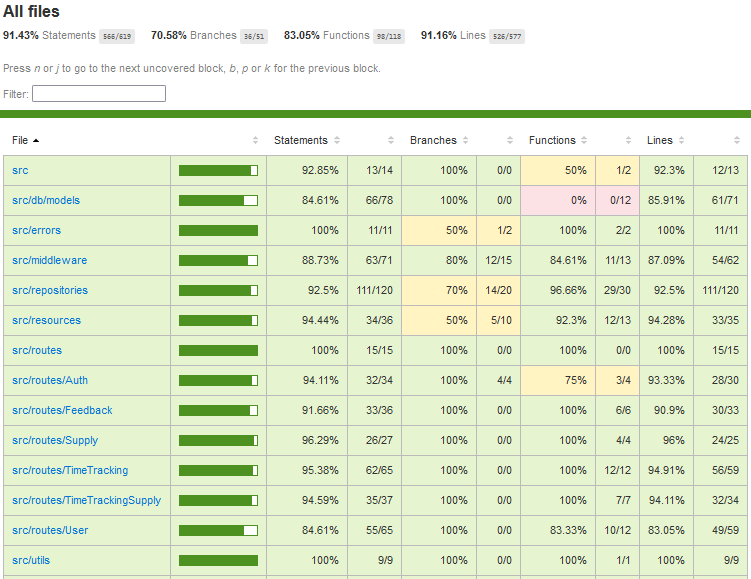
\includegraphics[scale=0.8]{./images/test-coverage.png}
  \caption{Copertura dei test suddivisa per file e directory.}
  \label{fig:coverage}
\end{figure}

La copertura complessiva del codice è stata misurata in termini di \textit{Statements}, \textit{Branches}, \textit{Functions} e \textit{Lines}. I risultati ottenuti sono i seguenti:

\begin{itemize}
  \item \textbf{Statements}: 91.43\% (566/619)
  \item \textbf{Branches}: 70.58\% (36/51)
  \item \textbf{Functions}: 83.05\% (98/118)
  \item \textbf{Lines}: 91.16\% (526/577)
\end{itemize}

Questi risultati indicano che la maggior parte del codice è stata coperta dai test, garantendo un elevato grado di affidabilità e robustezza dell'applicativo.





L'analisi della copertura dei test ha evidenziato un'ottima copertura complessiva del codice. Tuttavia, sono state identificate alcune aree con una copertura inferiore, specialmente nei rami condizionali (\textit{Branches}), dove è presente una copertura del 70.58\%. Queste aree rappresentano possibili punti di miglioramento, suggerendo la necessità di aggiungere ulteriori test per coprire scenari non ancora testati.

Nel complesso, la copertura ottenuta fornisce una solida base per garantire la qualità del codice e la stabilità dell'applicativo nel tempo.

\section{Pipeline CI/CD}

Ogni modifica al codice sorgente attiva la pipeline, che esegue una serie di operazioni per garantire che il nuovo codice sia correttamente integrato e che l'applicativo sia sempre in uno stato di rilascio pronto per la produzione.

\subsection{Struttura della Pipeline}

La pipeline è suddivisa in tre stage principali: \textbf{Installazione delle dipendenze}, \textbf{Test} e \textbf{Build del frontend}. Questi stage assicurano che le dipendenze necessarie siano installate correttamente, che il codice sia testato a fondo, e che il frontend venga costruito e sia pronto per la distribuzione.

\subsubsection{Stage 1: Installazione delle Dipendenze}

\begin{itemize}
  \item \textbf{Installazione delle dipendenze backend}: Viene eseguita all'interno di un container Docker basato sull'immagine \texttt{node:14}. Si naviga nella directory del backend e si installano le dipendenze tramite \texttt{npm install}. Le dipendenze vengono poi salvate come artefatti per gli stage successivi.
  \item \textbf{Installazione delle dipendenze frontend}: Simile al processo per il backend, viene eseguito \texttt{npm install} nella directory del frontend. Anche queste dipendenze vengono salvate come artefatti per l'uso successivo.
\end{itemize}

\subsubsection{Stage 2: Test}

Dopo aver installato le dipendenze del backend, la pipeline procede con l'esecuzione dei test. Durante questa fase:

\begin{itemize}
  \item Viene eseguito il comando \texttt{npm test} nella directory del backend per eseguire tutti i test unitari e di integrazione definiti.
  \item I test sono essenziali per garantire che le modifiche al codice non introducano regressioni o nuovi bug.
\end{itemize}

\subsubsection{Stage 3: Build del Frontend}

Una volta che tutte le dipendenze sono state installate e i test superati, la pipeline procede con la fase di build del frontend. Durante questa fase:

\begin{itemize}
  \item Viene eseguito il comando \texttt{npm run build} nella directory del frontend per creare una versione ottimizzata e pronta per la produzione dell'applicativo frontend.
  \item I file di build risultanti vengono salvati come artefatti, pronti per essere utilizzati nelle fasi successive, come il deployment.
\end{itemize}

\subsection{Flusso della Pipeline}

Ogni volta che viene effettuata una modifica al codice sorgente (ad esempio, un commit o una pull request), la pipeline viene attivata automaticamente (Figura \ref{fig:pipeline}).

\begin{figure}[ht]
  \centering
  \smartdiagram[flow diagram:horizontal]{
    Modifica Codice Sorgente,
    Installazione Dipendenze Backend,
    Installazione Dipendenze Frontend,
    Esecuzione Test Backend,
    Build del Frontend,
    Artefatti pronti per il Deployment
  }
  \caption{Flusso della Pipeline CI/CD.}
  \label{fig:pipeline}
\end{figure}



La pipeline CI/CD automatizza l'intero processo di integrazione, testing e distribuzione del codice, garantendo che ogni modifica sia testata e che il frontend sia sempre pronto per essere distribuito. La struttura modulare della pipeline permette di aggiungere facilmente ulteriori stage, come il deployment, per adattarsi alle necessità del progetto.


\chapter{Conclusioni}

In questo capitolo vengono presentate le conclusioni del progetto. In particolare vengono presentati i risulatati ottenuti, successivamente si evidenziano alcuni errori conosciuti e limitazioni attuali. Infine si esplorano le possibili implementazioni future per migliorare ulteriormente il sistema.

\section{Risultati}

Tutti i requisiti stabiliti durante la fase di progettazione sono stati pienamente soddisfatti, garantendo che il sistema rispondesse alle esigenze del partner di progetto.

\subsection{Registrazione delle Presenze}

La funzionalità di registrazione delle presenze, essenziale per il monitoraggio delle attività dei dipendenti, è stata implementata utilizzando il QR code. I dipendenti possono timbrare il loro arrivo e la loro partenza presso i clienti, e queste informazioni vengono immediatamente registrate nel sistema, garantendo un monitoraggio accurato e in tempo reale.

\subsection{Segnalazioni di Anomalie}

I dipendenti hanno la possibilità di segnalare qualsiasi anomalia riscontrata durante l'esecuzione dei servizi presso i clienti. Questa funzionalità consente di fornire una documentazione delle problematiche che possono essere esaminate dai responsabili per una rapida risoluzione.

\subsection{Ordini di Attrezzature e Prodotti}

È stata integrata la funzionalità per permettere ai dipendenti di ordinare attrezzature e prodotti direttamente tramite l'applicazione. Questo processo ottimizza la gestione delle scorte, assicurando che il personale disponga sempre del materiale necessario per svolgere i propri compiti.

\subsection{Verifica delle Timbrature da parte dei Responsabili}

I responsabili possono accedere a un'interfaccia dedicata per verificare le timbrature dei dipendenti, garantendo che i servizi siano eseguiti nei tempi previsti e con la qualità richiesta. Questa funzionalità è fondamentale per mantenere un elevato livello di controllo e supervisione.

\subsection{Funzionalità per i Clienti}

I clienti possono segnalare criticità nei servizi ricevuti. Questa funzionalità offre un canale diretto per il feedback dei clienti, fornendo all'azienda informazioni preziose per il miglioramento continuo.

\section{Errori Conosciuti}

Nonostante il successo complessivo del progetto, sono stati identificati alcuni errori e limitazioni che necessitano di ulteriori miglioramenti.

\subsection{Gestione degli Errori a Frontend}

Attualmente, la gestione degli errori a livello di frontend non è completamente ottimizzata. Gli utenti potrebbero non ricevere feedback adeguato in caso di problemi, come errori di rete o malfunzionamenti nelle richieste API. Questo aspetto richiede un'attenzione particolare per migliorare l'esperienza utente e la robustezza dell'applicazione.

\subsection{Design dell'App per i Dispositivi Mobili (User Experience)}

L'interfaccia utente dell'applicazione, sebbene funzionale, non è completamente ottimizzata per l'uso su dispositivi mobili. Alcuni elementi grafici e interazioni non sono ancora perfettamente adattati per schermi di piccole dimensioni, il che può influire negativamente sull'esperienza utente.

\subsection{Pannello di Gestione Utenti per gli Amministratori}

Nel pannello amministrativo per la gestione degli utenti, mancano alcune funzionalità chiave, come la possibilità di modificare l'indirizzo degli utenti di tipo cliente. Questa limitazione riduce la flessibilità degli amministratori nella gestione completa dei dati utente.

\section{Possibili Implementazioni Future}

Per migliorare ulteriormente il sistema e arricchirlo con nuove funzionalità, sono state identificate alcune possibili implementazioni future.

\subsection{Aggiunta di Gruppi per i Lavoratori}

Si propone di introdurre la possibilità di creare gruppi di lavoratori associati a specifici servizi. Questa funzionalità permetterebbe di creare una sorta di "stanza" virtuale in cui i membri del gruppo possono comunicare e scambiarsi informazioni relative al servizio a cui sono assegnati, migliorando la coordinazione e l'efficienza operativa.

\subsection{Feedback Mirati ai Servizi}

Implementare una funzionalità che consenta ai clienti di fornire feedback specifici sui servizi ricevuti, associati ai gruppi di lavoratori. Questo tipo di feedback mirato permetterebbe di ottenere valutazioni dettagliate e di intervenire in modo più preciso per migliorare la qualità del servizio.

\subsection{Comunicazione tra Lavoratori, Supervisori e Admin}

L'integrazione di una funzionalità di chat permetterebbe una comunicazione diretta tra lavoratori, supervisori e amministratori. Questo strumento migliorerebbe la gestione delle problematiche operative e faciliterebbe il coordinamento tra i vari attori coinvolti.

\subsection{Possibilità per i Lavoratori di Scattare Foto sul Luogo del Cliente}

Una funzionalità che consentirebbe ai lavoratori di scattare e caricare foto direttamente dall'app mentre si trovano presso il cliente sarebbe un'aggiunta preziosa. Questo permetterebbe di documentare visivamente lo stato del lavoro o eventuali anomalie riscontrate, migliorando la trasparenza e il controllo qualità del servizio erogato.


\cite{4538384}
\bibliographystyle{unsrt}
\bibliography{bibliografia}
\end{document}
